\documentclass{report}
\usepackage[margin=1in, paperwidth=8.5in, paperheight=11in]{geometry}
%Math packages%
\usepackage{amsmath}
\usepackage{amsthm}
%Spacing%
\usepackage{setspace}
\onehalfspacing
%Lecture number%
\newcommand{\lectureNum}{11}
%Variables - Date and Course%
\newcommand{\curDate}{February 7, 2017}
\newcommand{\course}{CS 240}
%Defining the example tag%
%\theoremstyle{definition}%
\newtheorem{ex}{Example}[section]
%Setting counter given the lecture number%
\setcounter{chapter}{\lectureNum{}}
%Package to insert code%
\usepackage{listings}
\usepackage{courier}
\usepackage{xcolor}
\lstset { 
    tabsize=2,
    breaklines=true,
    language=C++,
    backgroundcolor=\color{blue!8}, % set backgroundcolor
    basicstyle=\footnotesize\ttfamily,% basic font setting
}
%Package to draw trees%
\usepackage{tikz}

\begin{document}
%Note title%
\begin{center}
\begin{Large}
\textsc{\course{} | Lecture \lectureNum{}}
\end{Large}
\end{center} 
\noindent \textit{Bartosz Antczak} \hfill
\textit{Instructor: Eric Schost} \hfill
\textit{\curDate{}}
\rule{\textwidth}{0.4pt}

% Actual Notes%
\section{Operations on Skip Lists}
Recall that a \textbf{skip list} for a set of $S$ items is a series of lists $S_0, S_1, \cdots, S_h$. It contains a two-dimensional collection of positions: \textit{levels} and \textit{towers}.
\begin{figure}[ht]
\begin{center}
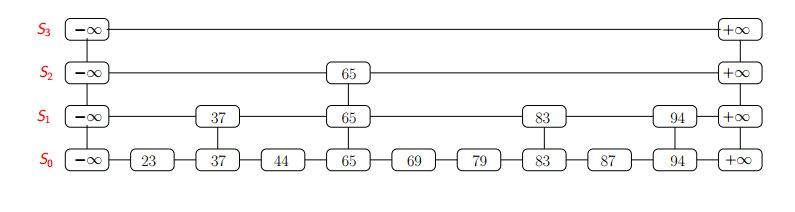
\includegraphics[scale=0.8]{skip-list.jpg}
\end{center}
\caption{The levels in this skip list are $S_3, S_2, S_1, S_0$. Taken from CS 240 course slides.}
\end{figure}
\subsection{Search}
The algorithm for search requires traversing the skip list. This is done by changing the position \texttt{p} in the skip list. Two methods that accomplish this are:
\begin{itemize}
\item \texttt{after(p)}: scans forward (i.e., moves to the successive tower)
\item \texttt{below(p)}: drops down one level in the tower
\end{itemize}
The algorithm is outlined as:
\begin{lstlisting}
skip-search(L,k)
// L: a skip list; k: a key
	p = topmost left position of L
	S = stack of positions, initially containing p
	while (below(p) != null)
		p = below(p)
		while (key(after(p)) < k)
			p = after(p)
		push p onto S
	return S
\end{lstlisting}
\subsection{Insert}
To insert an element \texttt{k} into the skip list, first determine the height of the new tower which contains the element. This is done by flipping a coin and letting \textit{i} denote the number of times the coin came up heads before the first tail. Then, insert the item into list $S_j$ after position $p_j$ for $0 \leq j \leq i$. This results in a tower of height $i$.
\begin{ex}
Inserting (52, v) into a skip list
\end{ex}
\begin{enumerate}
\item Flip a coin. Let's say  we get 1 head before the first tail (i.e., $i=1$). This means that the tower containing the key value 52 will be in $S_0$ and $S_1$.
\item Find the right-most position where we can insert 52 (since the skip list is sorted from left to right)
\item Insert the new tower of 52's into the list
\end{enumerate}
\begin{figure}[ht]
\begin{center}
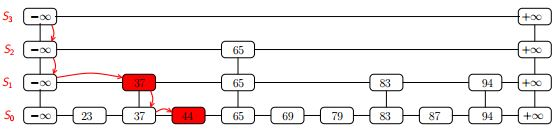
\includegraphics[scale=0.7]{insert1.jpg}
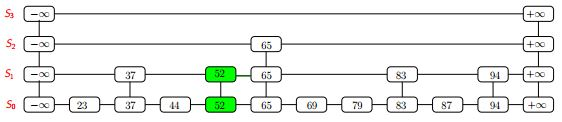
\includegraphics[scale=0.7]{insert2.jpg}
\end{center}
\caption{Example 11.1.1. Taken from CS 240 course slides.}
\end{figure}
\subsection{Delete}
To delete, search for \texttt{k} in the skip list and find all positions $p_0, p_1, \cdots, p_i$ of the items with the largest key smaller than \texttt{k}, where $p_j$ is in list $S_j$. Then for each $i$, if \texttt{key(after($p_i$)) == k}, then remove \texttt{after($p_i$)} from the list $S_i$. Lastly, remove all but one of the lists $S_i$ that contain only the two special keys.
\subsection{Summary of Skip Lists}
Skip lists are fast and simple to implement. The expected space usage is $O(n)$ with a height of $O(\log n)$. The expected runtimes for all of the previously defined methods are $O(\log n)$.
\subsubsection{Proof of Expected Height}
The probability that $S_i$ has one element at tower $j$ is $$\frac{1}{2^i}$$
For example, $S_0$ always has one element at tower $j$, so the probability is 1. If we move up one level to $S_1$, then the probability is halved.\\ 
From this, we can calculate the expected number of elements in
\begin{itemize}
\item each tower $j$: $\displaystyle \sum_{i \geq 0} \frac{1}{2^i} = 2$
\item each row $S_i$: $\displaystyle \frac{n}{2^i}$
\item in the entire skip list: $2n$
\end{itemize}
Let's define an indicator variable $V_i$, $i \geq 1$ by
$$V_i = 
     \begin{cases}
      0 & \text{if } S_i \text{ is empty} \\
      1 & \text{otherwise} \\ 
     \end{cases} $$
This means that the height of the skip list is $\displaystyle \sum_{i \geq 1} V_i$. This means that the expected height $E(h)$ of the skip list is $$\sum_{i\geq 1} E(V_i)$$
Two things to note here:
\begin{itemize}
\item We always have $E(V_i) \leq 1$
\item We also have that $V_i$ is less than or equal to the number of elements in $S_i$: $$E(V_i) \leq E(S_i) = \frac{n}{2^i}$$
\end{itemize}
So, 
\begin{align*}
E(h) &= \sum_{i \geq 1}^\infty E(V_i) \\
&= \sum_{i \geq 1}^{\log_2 (n)}E(V_i) + \sum_{i > \log_2(n)}^\infty E(V_i) \\
&\leq \sum_{i \geq 1}^{\log_2 (n)} 1 + \sum_{i > \log_2(n)}^\infty \frac{n}{2^i} \\
&= \log (n) + 1 & \text{}
\end{align*}
Thus, the expected height $V_i$ is indeed in $O(\log n)$.
\subsubsection{Proof of Expected Time for Search}
Call $C(k)$ the expected length of a path that goes backward $k$ levels up: $$C(k) = \frac{1}{2}[1 + C(k-1)] + \frac{1}{2}[1+C(k)]$$
The $+1$ represents the step up and $C(k-1)$ represents the number of levels to go. Simplifying, we get
\begin{align*}
C(k) &= 2 + C(k-1) \\
&= 2 + 2 + C(k-2) \\
&= 2 + 2 + \cdots + C(0) & (C(0)\text{ is zero)} \\
&= 2k
\end{align*}
Thus, $C(k) \in O(k)$, which means that the expected length of a search is $C(k) \in O(\log n)$.
%END%
\end{document}